\documentclass{article}
\usepackage{fullpage}
\usepackage{graphicx}
\usepackage{float}
\usepackage{subfig}
\usepackage{verbatim}
\newcommand{\proxypacurl}{https://iodine.tjhsst.edu/www/proxy.pac}
\newcommand{\librarydbpage}{http://www.tjhsst.edu/curriculum/library/wordpress/databases/}
\author{Andrew Hamilton\\
{\small Network / Systems Administrator}\\
{\small TJHSST IT Team}\\
{\small ahamilto@tjhsst.edu}}
\title{TJHSST Zeus Database Proxy Handbook\\
{\small Revision 2.0 (August 30, 2012)}}
\begin{document}
\maketitle
\tableofcontents
\begin{flushleft}
\section{Internet Explorer 9 on Windows Vista/7}
\begin{enumerate}
\item Launch Internet Explorer 9
\item Clear your IE9 page cache
\item In the upper right corner of IE9, click on the \textbf{gear icon} (see Figure \ref{fig:windows-ie9-internetoptions})
\item In the menu that appears, click on \textbf{Internet Options} (see Figure \ref{fig:windows-ie9-internetoptions})
\item IE9 will open the \textbf{Internet Options} window
\item In the \textbf{Internet Options} window, click on the \textbf{Connections} tab at the top (see Figure \ref{fig:windows-ie9-connectionoptions})
\item At the bottom of the \textbf{Connections} tab, click on the \textbf{LAN Settings} button. (see Figure \ref{fig:windows-ie9-connectionoptions})
\item IE9 will open the \textbf{Local Area Network (LAN) Settings} window
\item In the \textbf{LAN Settings} window, check the box next to \textbf{Use automatic configuration script} (see Figure \ref{fig:windows-ie9-lansettings})
\item In the \textbf{Address} box underneath \textbf{Use automatic configuration script}, put in \linebreak\textbf{\proxypacurl} (see Figure \ref{fig:windows-ie9-lansettings})
\item Click the \textbf{OK} button at the bottom of the \textbf{LAN Settings} window, then click the \textbf{OK} button at the bottom of the \textbf{Internet Options} window
\item Go to the webpage \textbf{\librarydbpage}
\item Click on the name of the database you wish to access
\item IE9 will bring up the \textbf{Windows Security} password prompt.
\item In the username field, enter LOCAL$\backslash$$<$yourusername$>$ eg. LOCAL$\backslash$2013awilliam and in the password field enter your TJ Password; the one you use to log in to Iodine. (see Figure \ref{fig:windows-ie9-passwdprompt})
\item Click the \textbf{OK} button on the password prompt
\item You should now have access to the TJHSST Library Databases.
\end{enumerate}
\begin{figure}[H]
\centering
\subfloat[Gear Menu]{\label{fig:windows-ie9-internetoptions}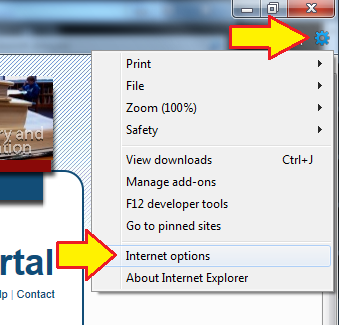
\includegraphics[height=60mm]{images/windows-ie9-internetoptions.png}}
\subfloat[Connection Options]{\label{fig:windows-ie9-connectionoptions}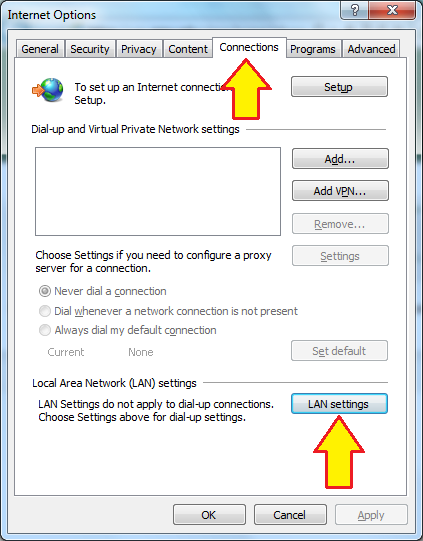
\includegraphics[height=90mm]{images/windows-connectionoptions.png}}
\caption{IE9 Proxy Configuration Part 1}
\end{figure}
\begin{figure}[H]
\centering
\subfloat[LAN Settings]{\label{fig:windows-ie9-lansettings}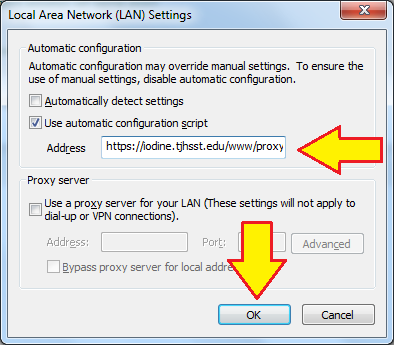
\includegraphics[height=70mm]{images/windows-lansettings.png}}
\subfloat[Password Prompt]{\label{fig:windows-ie9-passwdprompt}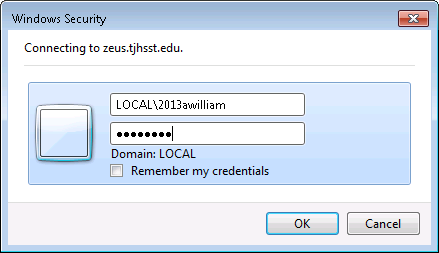
\includegraphics[height=45mm]{images/windows-ie9-passwdprompt.png}}
\caption{IE9 Proxy Configuration Part 2}
\end{figure}
\section{Internet Explorer 8 on Windows XP}
\begin{enumerate}
\item Launch Internet Explorer 8
\item Clear your IE8 page cache
\item In the upper right corner of IE8, click on the \textbf{Tools} menu (see Figure \ref{fig:windows-ie8-internetoptions})
\item In the menu that appears, click on \textbf{Internet Options} (see Figure \ref{fig:windows-ie8-internetoptions})
\item IE8 will open the \textbf{Internet Options} window
\item In the \textbf{Internet Options} window, click on the \textbf{Connections} tab at the top (see Figure \ref{fig:windows-ie8-connectionoptions})
\item At the bottom of the \textbf{Connections} tab, click on the \textbf{LAN Settings} button. (see Figure \ref{fig:windows-ie8-connectionoptions})
\item IE8 will open the \textbf{Local Area Network (LAN) Settings} window
\item In the \textbf{LAN Settings} window, check the box next to \textbf{Use automatic configuration script} (see Figure \ref{fig:windows-ie8-lansettings})
\item In the \textbf{Address} box underneath \textbf{Use automatic configuration script}, put in \linebreak\textbf{\proxypacurl} (see Figure \ref{fig:windows-ie8-lansettings})
\item Click the \textbf{OK} button at the bottom of the \textbf{LAN Settings} window, then click the \textbf{OK} button at the bottom of the \textbf{Internet Options} window
\item Go to the webpage \textbf{\librarydbpage}
\item Click on the name of the database you wish to access
\item IE8 will bring up the \textbf{Windows Security} password prompt.
\item In the username field, enter LOCAL$\backslash$$<$yourusername$>$ eg. LOCAL$\backslash$2013awilliam and in the password field enter your TJ Password; the one you use to log in to Iodine. (see Figure \ref{fig:windows-ie8-passwdprompt})
\item Click the \textbf{OK} button on the password prompt
\item You should now have access to the TJHSST Library Databases.
\end{enumerate}
\begin{figure}[H]
\centering
\subfloat[Tools Menu]{\label{fig:windows-ie8-internetoptions}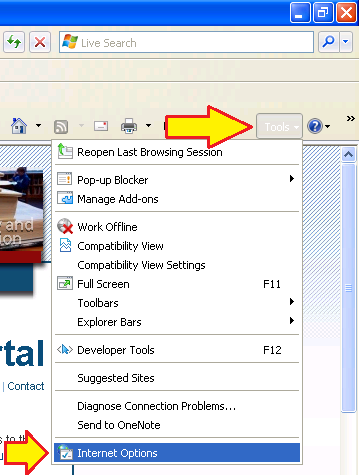
\includegraphics[height=80mm]{images/windows-ie8-internetoptions.png}}
\subfloat[Connection Options]{\label{fig:windows-ie8-connectionoptions}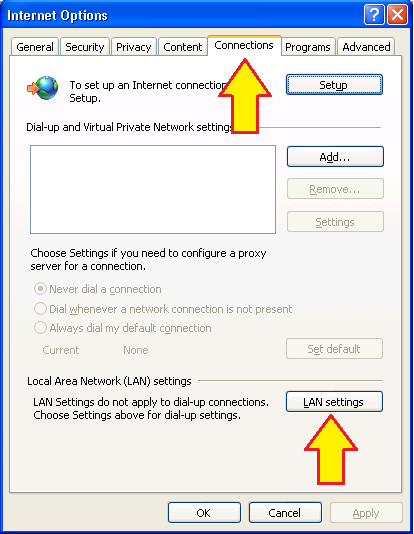
\includegraphics[height=80mm]{images/windows-ie8-connectionoptions.png}}
\caption{IE8 Proxy Configuration Part 1}
\end{figure}
\begin{figure}[H]
\centering
\subfloat[LAN Settings]{\label{fig:windows-ie8-lansettings}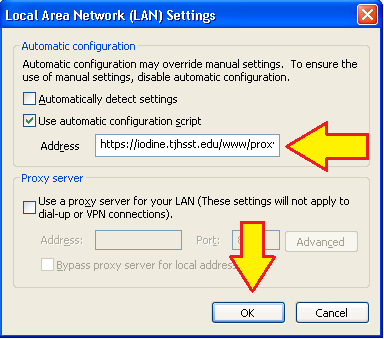
\includegraphics[height=70mm]{images/windows-ie8-lansettings.png}}
\subfloat[Password Prompt]{\label{fig:windows-ie8-passwdprompt}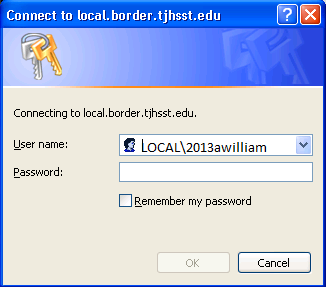
\includegraphics[height=45mm]{images/windows-ie8-passwdprompt.png}}
\caption{IE8 Proxy Configuration Part 2}
\end{figure}
\section{Mozilla Firefox 5$+$ on Windows}
\begin{enumerate}
\item Launch Mozilla Firefox
\item Clear your Firefox page cache
\item In the upper left corner of Firefox, click on the \textbf{Firefox} menu (see Figure \ref{fig:windows-firefox-optionsmenu})
\item In the menu that appears, click on \textbf{Options} button (see Figure \ref{fig:windows-firefox-optionsmenu})
\item Firefox will open the \textbf{Options} window
\item In the \textbf{Options} window, click on the \textbf{Advanced} tab at the top; then click on the \textbf{Network} tab that appears below it (see Figure \ref{fig:windows-firefox-advancednetwork})
\item At the top of the \textbf{Network} tab, click on the \textbf{Settings} button in the \textbf{Connections} section (see Figure \ref{fig:windows-firefox-advancednetwork})
\item Firefox will open the \textbf{Connection Settings} window
\item In the \textbf{Connection Settings} window, check the radio button next to \textbf{Automatic proxy configuration URL} (see Figure \ref{fig:windows-firefox-connectionsettings})
\item In the address box underneath \textbf{Automatic proxy configuration URL}, put in \linebreak\textbf{\proxypacurl} (see Figure \ref{fig:windows-ie8-lansettings})
\item Click the \textbf{OK} button at the bottom of the \textbf{Connection Settings} window, then click the \textbf{OK} button at the bottom of the \textbf{Options} window
\item Go to the webpage \textbf{\librarydbpage}
\item Click on the name of the database you wish to access
\item Firefox will bring up the \textbf{Authentication Required} password prompt.
\item In the username field, enter LOCAL$\backslash$$<$yourusername$>$ eg. LOCAL$\backslash$2013awilliam and in the password field enter your TJ Password; the one you use to log in to Iodine. (see Figure \ref{fig:windows-firefox-passwdprompt})
\item Click the \textbf{OK} button on the password prompt
\item You should now have access to the TJHSST Library Databases.
\end{enumerate}
\begin{figure}[H]
\centering
\subfloat[Options Menu]{\label{fig:windows-firefox-optionsmenu}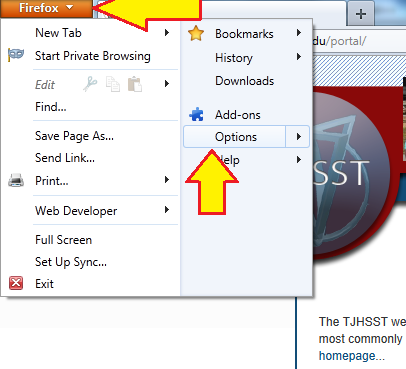
\includegraphics[height=60mm]{images/windows-firefox-optionsmenu.png}}
\subfloat[Advanced Network Options]{\label{fig:windows-firefox-advancednetwork}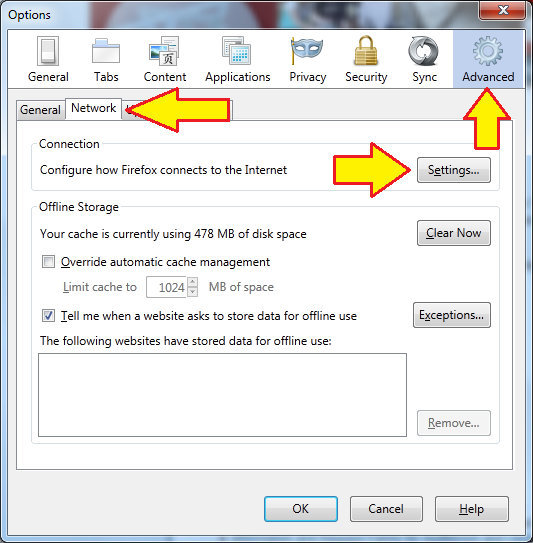
\includegraphics[height=90mm]{images/windows-firefox-advancednetwork.png}}
\caption{Firefox on Windows Proxy Configuration Part 1}
\end{figure}
\begin{figure}[H]
\centering
\subfloat[Connection Settings]{\label{fig:windows-firefox-connectionsettings}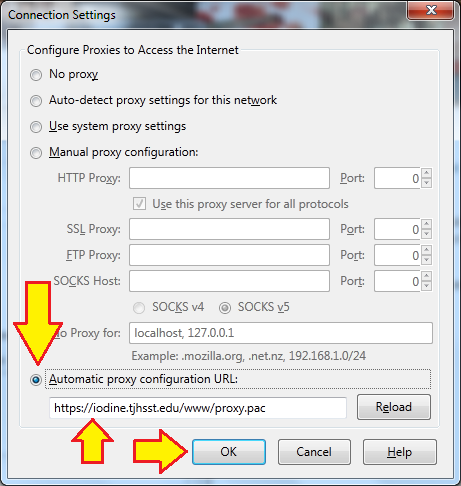
\includegraphics[height=70mm]{images/windows-firefox-connectionsettings.png}}
\subfloat[Password Prompt]{\label{fig:windows-firefox-passwdprompt}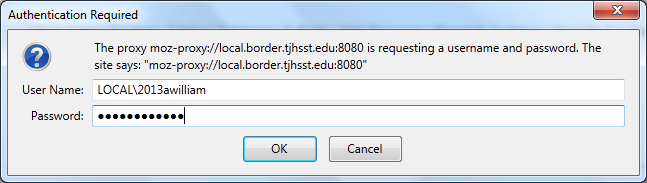
\includegraphics[height=25mm]{images/windows-firefox-passwdprompt.png}}
\caption{Firefox on Windows Proxy Configuration Part 2}
\end{figure}
\section{Mozilla Firefox 5$+$ on OS X}
\begin{enumerate}
\item Launch Mozilla Firefox
\item Clear your Firefox page cache
\item In the upper left corner of the scren, click on the \textbf{Firefox} menu (see Figure \ref{fig:osx-firefox-preferences})
\item In the menu that appears, click on \textbf{Preferences} button (see Figure \ref{fig:osx-firefox-preferences})
\item Firefox will open the \textbf{Preferences} window
\item In the \textbf{Preferences} window, click on the \textbf{Advanced} tab at the top; then click on the \textbf{Network} tab that appears below it (see Figure \ref{fig:osx-firefox-advancednetwork})
\item At the top of the \textbf{Network} tab, click on the \textbf{Settings} button in the \textbf{Connections} section (see Figure \ref{fig:osx-firefox-advancednetwork})
\item Firefox will open the \textbf{Connection Settings} window
\item In the \textbf{Connection Settings} window, check the radio button next to \textbf{Automatic proxy configuration URL} (see Figure \ref{fig:osx-firefox-connectionsettings})
\item In the address box underneath \textbf{Automatic proxy configuration URL}, put in \linebreak\textbf{\proxypacurl} (see Figure \ref{fig:osx-firefox-connectionsettings})
\item Click the \textbf{OK} button at the bottom of the \textbf{Connection Settings} window, then click the red \textbf{X} button in the upper left corner of the \textbf{Preferences} window
\item Go to the webpage \textbf{\librarydbpage}
\item Click on the name of the database you wish to access
\item Firefox will bring up the \textbf{Authentication Required} password prompt.
\item In the username field, enter LOCAL$\backslash$$<$yourusername$>$ eg. LOCAL$\backslash$2013awilliam and in the password field enter your TJ Password; the one you use to log in to Iodine. (see Figure \ref{fig:osx-firefox-passwdprompt})
\item Click the \textbf{OK} button on the password prompt
\item You should now have access to the TJHSST Library Databases.
\end{enumerate}
\begin{figure}[H]
\centering
\subfloat[Preferences Menu]{\label{fig:osx-firefox-preferences}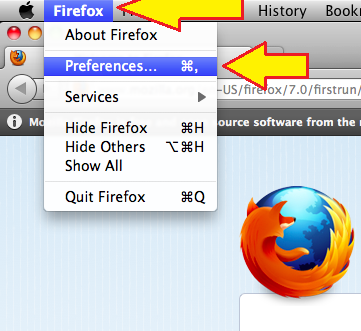
\includegraphics[height=40mm]{images/osx-firefox-preferences.png}}
\subfloat[Advanced Network Options]{\label{fig:osx-firefox-advancednetwork}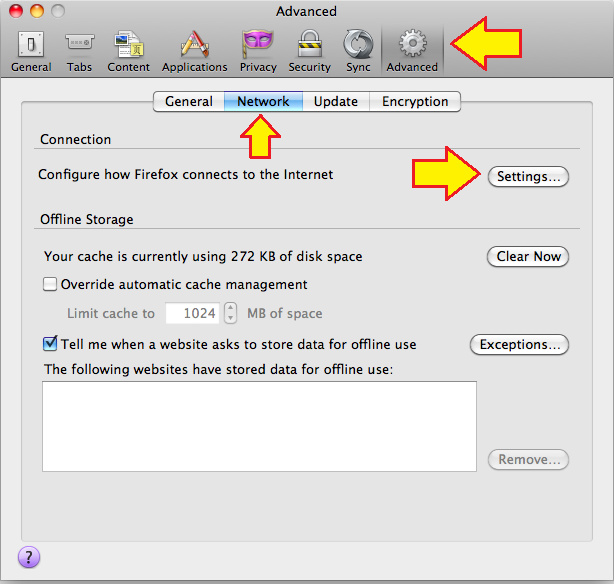
\includegraphics[height=90mm]{images/osx-firefox-advancednetwork.png}}
\caption{Firefox on OS X Proxy Configuration Part 1}
\end{figure}
\begin{figure}[H]
\centering
\subfloat[Connection Settings]{\label{fig:osx-firefox-connectionsettings}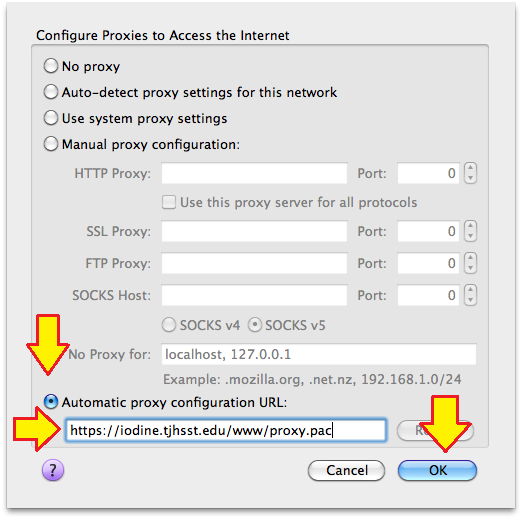
\includegraphics[height=70mm]{images/osx-firefox-connectionsettings.png}}
\subfloat[Password Prompt]{\label{fig:osx-firefox-passwdprompt}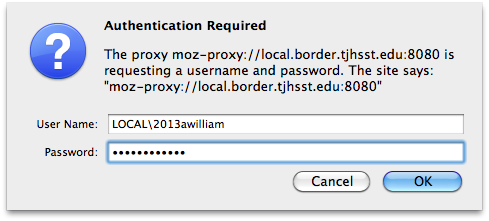
\includegraphics[height=25mm]{images/osx-firefox-passwdprompt.png}}
\caption{Firefox on OS X Proxy Configuration Part 2}
\end{figure}
%\section{Mozilla Firefox 5$+$ on Linux}
%\section{Apple Safari on Windows}
\section{Apple Safari on OS X}
\begin{enumerate}
\item Launch Safari
\item Clear your Safari page cache
\item In the upper left corner, click on the \textbf{Safari} menu (see Figure \ref{fig:osx-safari-preferences})
\item In the menu that appears, click on \textbf{Preferences} (see Figure \ref{fig:osx-safari-preferences})
\item Safari will open the \textbf{Preferences} window
\item in the \textbf{Preferences} window, click on the \textbf{Advanced} tab at the top (see Figure \ref{fig:osx-safari-advanced})
\item At the bottom of the \textbf{Advanced} tab, click on the \textbf{Change Setttings...} button in the \textbf{Proxies} section (see Figure \ref{fig:osx-safari-advanced})
\item Safari will open the \textbf{Proxies} windows
\item In the \textbf{Proxies} window, check the box next to \textbf{Automatic Proxy Configuration} (see Figure \ref{fig:osx-safari-proxies})
\item In the \textbf{URL} box on the right, put in \linebreak\textbf{\proxypacurl} (see Figure \ref{fig:osx-safari-proxies})
\item Click on the \textbf{OK} button at the bottom of the \textbf{Proxies} window, then click the red \textbf{X} button in the upper left hand corner of the \textbf{Advanced} window.
\item Go to the webpage \textbf{\librarydbpage}
\item Click on the name of the database you wish to access
\item Safari will bring up the \textbf{Safari password prompt}.
\item In the username field, enter LOCAL$\backslash$$<$yourusername$>$ eg. LOCAL$\backslash$2013awilliam and in the password field enter your TJ Password; the one you use to log in to Iodine. (see Figure \ref{fig:osx-safari-passwdprompt})
\item Click the \textbf{Log In} button on the password prompt
\item You should now have access to the TJHSST Library Databases.
\end{enumerate}
\begin{figure}[H]
\centering
\subfloat[Preferences Menu]{\label{fig:osx-safari-preferences}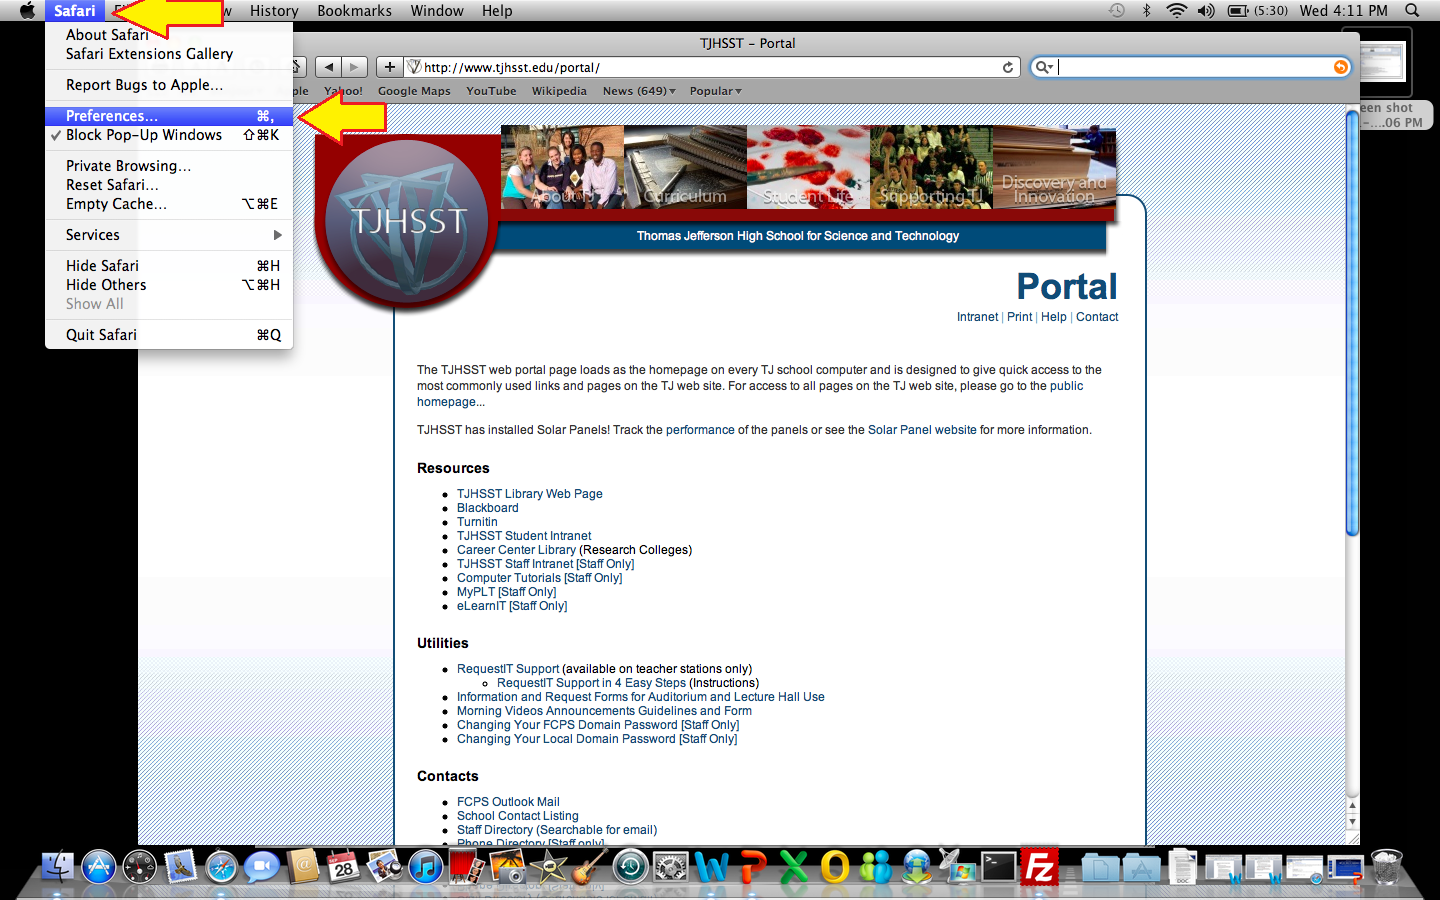
\includegraphics[height=50mm]{images/osx-safari-preferences.png}}
\subfloat[Advanced Options]{\label{fig:osx-safari-advanced}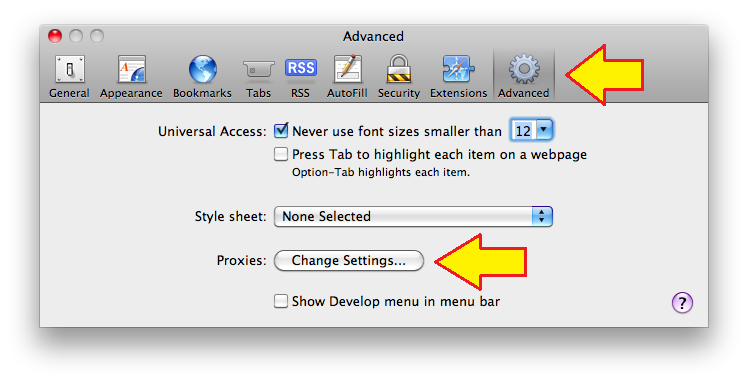
\includegraphics[height=40mm]{images/osx-safari-advanced.png}}
\caption{Safari on OS X Proxy Configuration Part 1}
\end{figure}
\begin{figure}[H]
\centering
\subfloat[Proxies]{\label{fig:osx-safari-proxies}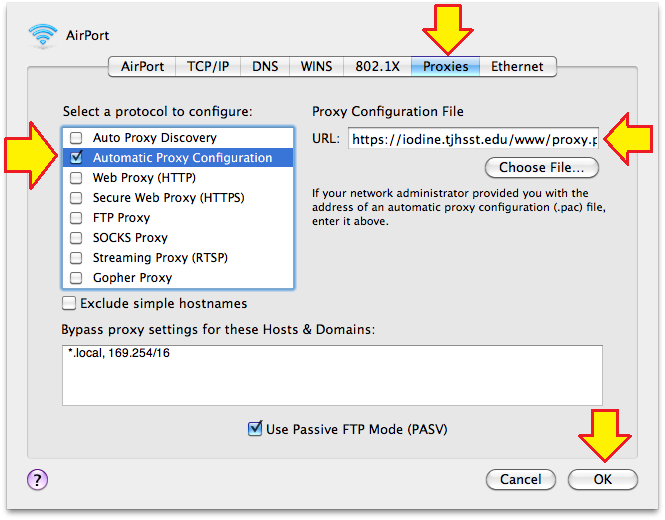
\includegraphics[height=70mm]{images/osx-proxies.png}}
\subfloat[Password Prompt]{\label{fig:osx-safari-passwdprompt}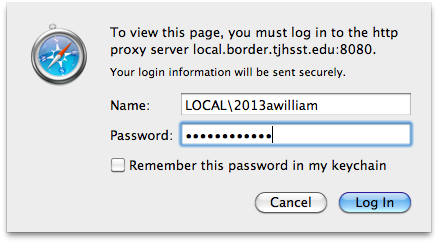
\includegraphics[height=30mm]{images/osx-safari-passwdprompt.png}}
\caption{Safari on OS X Proxy Configuration Part 2}
\end{figure}
\section{Google Chrome on Windows}
\begin{enumerate}
\item Launch Google Chrome
\item Clear your Chrome page cache
\item In the upper right corner of Chrome, click on the \textbf{wrench} menu (see Figure \ref{fig:windows-chrome-optionsmenu})
\item In the menu that appears, click on \textbf{Options} (see Figure \ref{fig:windows-chrome-optionsmenu})
\item Chrome will open the \textbf{Options} tab
\item In the \textbf{Options} tab, click on the \textbf{Under the Hood} tab on the left (see Figure \ref{fig:windows-chrome-underthehood})
\item At the bottom of the \textbf{Under the Hood} tab, click on the \textbf{Change proxy settings} button in the \textbf{Network} section (see Figure \ref{fig:windows-chrome-underthehood})
\item Chrome will open the \textbf{Internet Options} window
\item At the bottom of the \textbf{Connections} tab, click on the \textbf{LAN Settings} button. (see Figure \ref{fig:windows-chrome-connectionoptions})
\item Chrome will open the \textbf{Local Area Network (LAN) Settings} window
\item In the \textbf{LAN Settings} window, check the box next to \textbf{Use automatic configuration script} (see Figure \ref{fig:windows-chrome-lansettings})
\item In the \textbf{Address} box underneath \textbf{Use automatic configuration script}, put in \linebreak\textbf{\proxypacurl} (see Figure \ref{fig:windows-chrome-lansettings})
\item Click the \textbf{OK} button at the bottom of the \textbf{LAN Settings} window, then click the \textbf{OK} button at the bottom of the \textbf{Internet Options} window
\item Go to the webpage \textbf{\librarydbpage}
\item Click on the name of the database you wish to access
\item Chrome will bring up the \textbf{Authentication Required} password prompt.
\item In the username field, enter LOCAL$\backslash$$<$yourusername$>$ eg. LOCAL$\backslash$2013awilliam and in the password field enter your TJ Password; the one you use to log in to Iodine. (see Figure \ref{fig:windows-chrome-passwdprompt})
\item Click the \textbf{OK} button on the password prompt
\item You should now have access to the TJHSST Library Databases.
\end{enumerate}
\begin{figure}[H]
\centering
\subfloat[Options Menu]{\label{fig:windows-chrome-optionsmenu}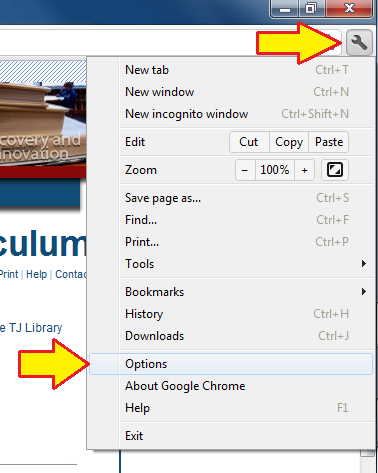
\includegraphics[height=50mm]{images/windows-chrome-optionsmenu.png}}
\subfloat[Under the Hood]{\label{fig:windows-chrome-underthehood}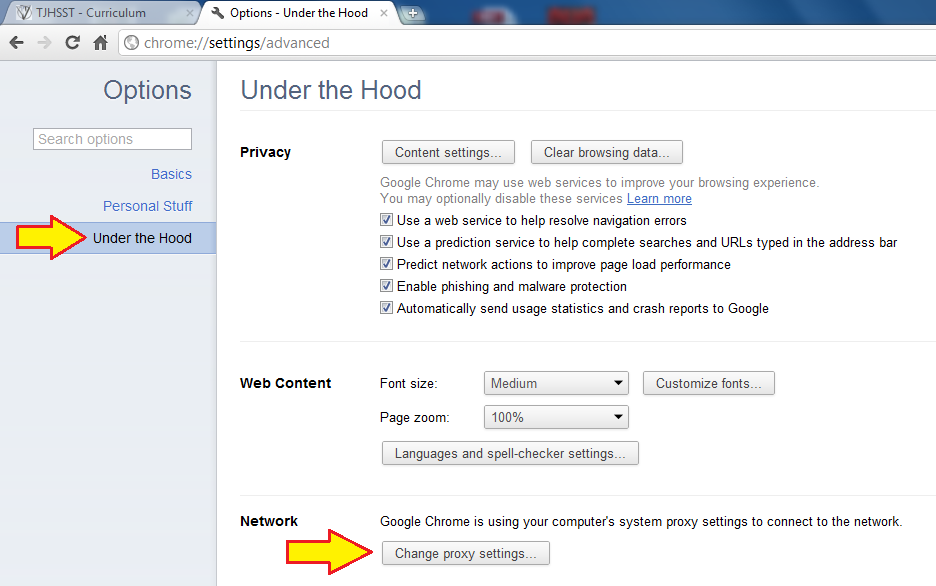
\includegraphics[height=70mm]{images/windows-chrome-underthehood.png}}
\caption{Chrome on Windows Proxy Configuration Part 1}
\end{figure}
\begin{figure}[H]
\centering
\subfloat[Internet Options]{\label{fig:windows-chrome-connectionoptions}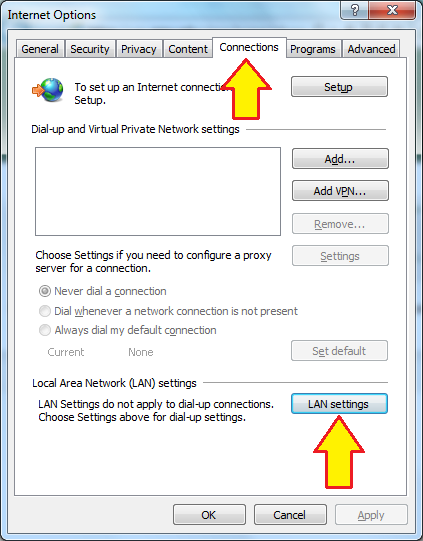
\includegraphics[height=50mm]{images/windows-connectionoptions.png}}
\subfloat[LAN Settings]{\label{fig:windows-chrome-lansettings}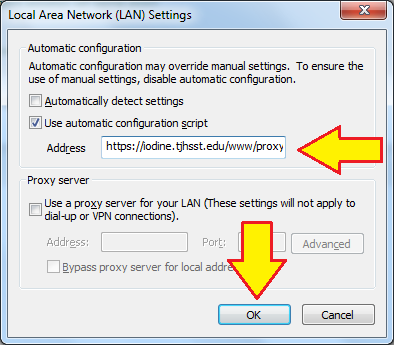
\includegraphics[height=60mm]{images/windows-lansettings.png}}
\subfloat[Password Prompt]{\label{fig:windows-chrome-passwdprompt}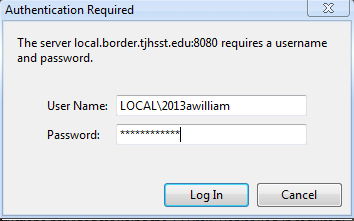
\includegraphics[height=30mm]{images/windows-chrome-passwdprompt.png}}
\caption{Chrome on Windows Proxy Configuration Part 2}
\end{figure}
\section{Google Chrome on OS X}
\begin{enumerate}
\item Launch Google Chrome
\item Clear your Chrome page cache
\item In the upper right corner of Chrome, click on the \textbf{wrench} menu (see Figure \ref{fig:osx-chrome-preferences})
\item In the menu that appears, click on \textbf{Preferences} (see Figure \ref{fig:osx-chrome-preferences})
\item Chrome will open the \textbf{Preferences} tab
\item In the \textbf{Preferences} tab, click on the \textbf{Under the Hood} tab on the left (see Figure \ref{fig:osx-chrome-underthehood})
\item At the bottom of the \textbf{Under the Hood} tab, click on the \textbf{Change proxy settings} button in the \textbf{Network} section (see Figure \ref{fig:osx-chrome-underthehood})
\item Chrome will open the \textbf{Proxies} windows
\item In the \textbf{Proxies} window, check the box next to \textbf{Automatic Proxy Configuration} (see Figure \ref{fig:osx-chrome-proxies})
\item In the \textbf{URL} box on the right, put in \linebreak\textbf{\proxypacurl} (see Figure \ref{fig:osx-chrome-proxies})
\item Click on the \textbf{OK} button at the bottom of the \textbf{Proxies} window
\item Go to the webpage \textbf{\librarydbpage}
\item Click on the name of the database you wish to access
\item Chrome will bring up the \textbf{Chome password prompt}.
\item In the username field, enter LOCAL$\backslash$$<$yourusername$>$ eg. LOCAL$\backslash$2013awilliam and in the password field enter your TJ Password; the one you use to log in to Iodine. (see Figure \ref{fig:osx-chrome-passwdprompt})
\item Click the \textbf{Log In} button on the password prompt
\item You should now have access to the TJHSST Library Databases.
\end{enumerate}
\begin{figure}[H]
\centering
\subfloat[Preferences Menu]{\label{fig:osx-chrome-preferences}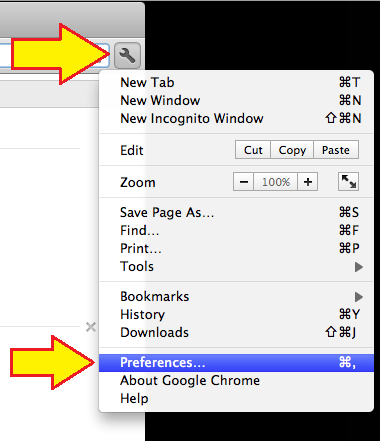
\includegraphics[height=50mm]{images/osx-chrome-preferences.png}}
\subfloat[Advanced Options]{\label{fig:osx-chrome-underthehood}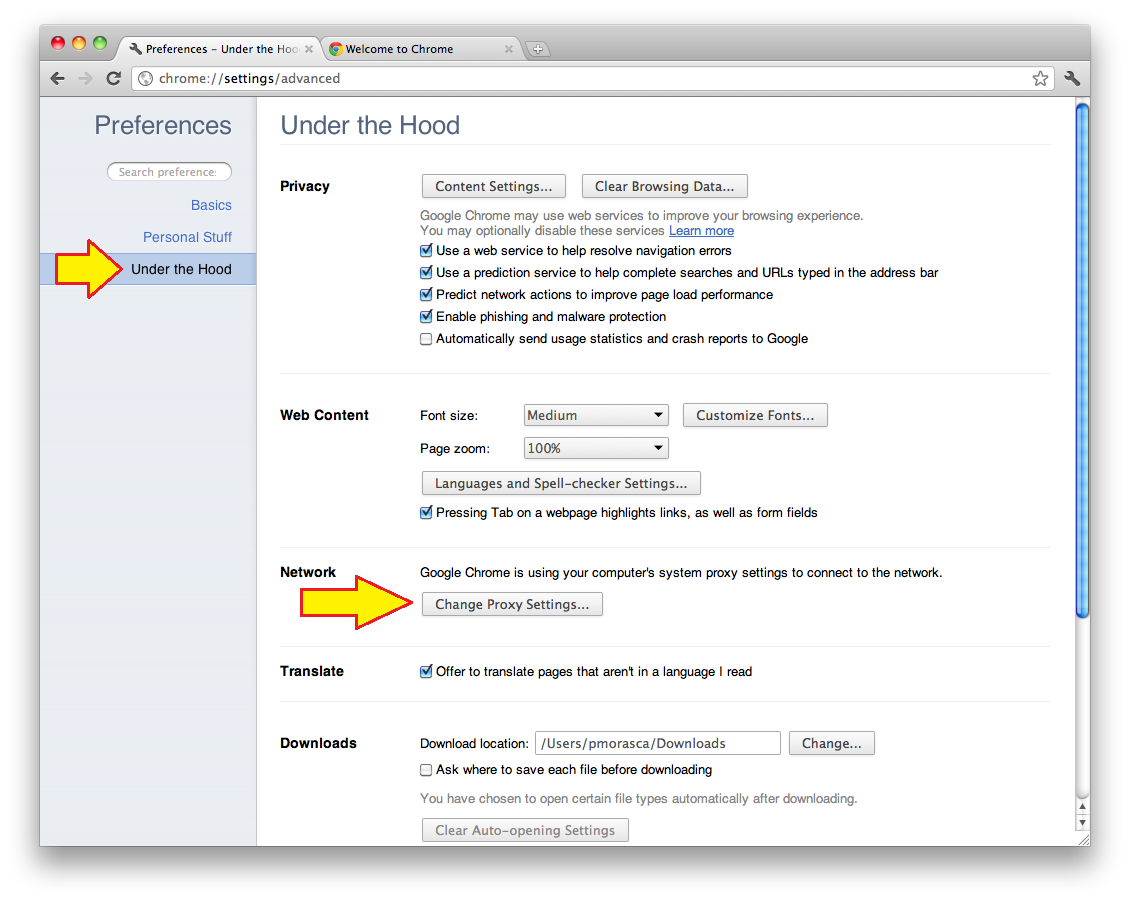
\includegraphics[height=70mm]{images/osx-chrome-underthehood.png}}
\caption{Chrome on OS X Proxy Configuration Part 1}
\end{figure}
\begin{figure}[H]
\centering
\subfloat[Proxies]{\label{fig:osx-chrome-proxies}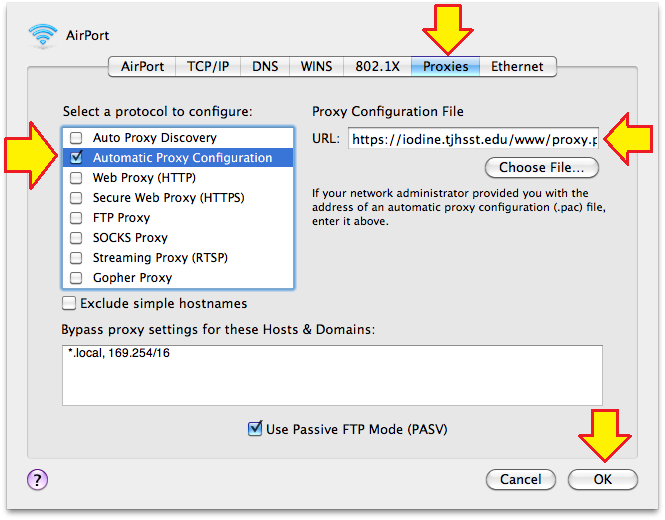
\includegraphics[height=70mm]{images/osx-proxies.png}}
\subfloat[Password Prompt]{\label{fig:osx-chrome-passwdprompt}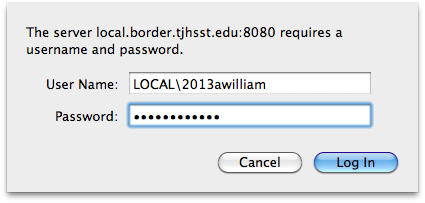
\includegraphics[height=30mm]{images/osx-chrome-passwdprompt.png}}
\caption{Chrome on OS X Proxy Configuration Part 2}
\end{figure}
%\section{Google Chromium on Linux}
%\section{Opera 11 on Windows}
%\section{Opera 11 on OS X}
%\section{Opera 11 on Linux}
\end{flushleft}
\end{document}
